\documentclass[a4paper,twoside,12pt]{article}

% Packages for table
\usepackage{rotating}
\usepackage{color}
\usepackage[table,xcdraw]{xcolor}
\definecolor{LightGray}{gray}{0.95}

\usepackage[T1]{fontenc}
\usepackage[utf8]{inputenc}
\usepackage[ngerman, english]{babel}

\usepackage[inner=1.5cm, outer=1cm, top=2cm, bottom=2cm]{geometry}
\usepackage[handwritten]{xcookybooky}

\usepackage{cancel}
\usepackage[export]{adjustbox}


\usepackage{hyperref}    % must be the last package
\hypersetup{%
    pdfauthor            = {Kilian Hähn, Ann-Kathrin Pullmann, Jonas Höchst},
    pdftitle             = {Kochbuch für das Landeslager},
    pdfsubject           = {Landeslager 2016},
    pdfkeywords          = {Landeslager, 2016, VCP, Kochbuch}
}

\hbadness=10000    % Ignore underfull boxes
\usepackage{helvet}
% \renewcommand{\familydefault}{\sfdefault}

\begin{document}
\thispagestyle{empty}
\begin{center}
    
\includegraphics[width=.2\linewidth, right]{Zeichen.pdf}
    % ~\\[1cm]
    ~\\[2cm]
    
\includegraphics[width=0.8\textwidth]{Badge-crop.pdf}
    ~\\[4cm] 
    
    % \normalsize{Landeslager 2016}\\
	\Huge{\textbf{Kochbuch}}\\
	{\large \textbf{Hessæhāven — Zeit zum Handeln}}\\
\end{center}
\clearpage

\section{Vorwort}

Hallo liebe Stammesköche,~\\
~\\
seid ihr schon aufgeregt? Wir schon! Damit auch wirklich nix schiefgeht und ihr genau wisst, was ihr mit den ganzen Zutaten, die ihr von uns bekommt, anfangen könnt, haben wir für euch dieses Kochbuch vorbereitet.\\
~\\
In den Rezepten stehen immer die Mengen für 10 Personen. Ihr müsst aber eigentlich eh nichts umrechnen – ihr kriegt ja von uns genau das, was ihr braucht. ~\\
~\\
Zu den Brotmahlzeiten gibt es immer Wurst, Käse, Aufstriche, Gemüse, Obst, etc. – wenn ihr merkt, dass ihr bspw. zu viel Wurst habt, sagt es uns. Wir heben sie im Kühlschrank für euch auf und wenn ihr sie erst abends braucht, bekommt ihr sie dann. ~\\
~\\
Wir alle wissen, dass man eine Menge Zeit in der Küche totschlägt, bis das Wasser kocht, die Kisten kommen oder alles geschnibbelt ist. Damits euch nicht zu lang wird, birgt dieses Kochbuch noch einiges mehr als Rezepte.~\\
~\\
Falls ihr Fragen oder Lob habt, wendet euch vertrauensvoll an uns. Falls ihr meckern wollt, geht woanders hin – zur Technik oder so.~\\
~\\
Wir sehn uns,~\\
~\\
~~~~~Jonas, Kilian \& Anni~\\
~\\
P.S.: Risotto ist der Hit

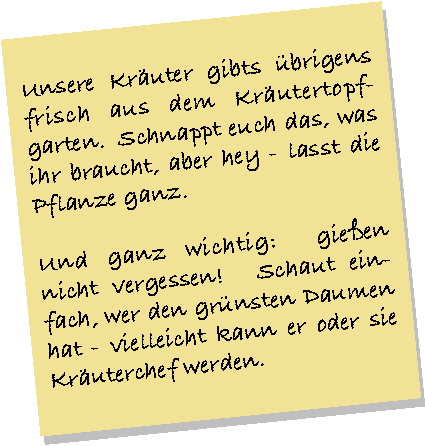
\includegraphics[right]{note-crop.pdf}

\renewcommand{\contentsname}{Inhaltsverzeichnis}
\tableofcontents

% \setBackgroundPicture[x, y=0, width=\paperwidth, height, orientation = pagecenter]{pic/Fingerprint}
\refstepcounter{section}
\addcontentsline{toc}{section}{\protect\numberline{\thesection}Rezepte}
\sectionmark{Rezepte}

\setHeadlines{
    inghead = Zutaten,
    prephead = Zubereitung,
    hinthead = Tipp,
}

%!TEX root = ../Kochbuch.tex

% Complete recipe example
\begin{recipe}[]{Porridge}
    \graph{
        big=pic/porridge,
        small=pic/hafer
    }
    
    % \introduction{%
    % ``Das ist vergleichsweise einfach, aber man muss viel schneiden.''\flushright --- \emph{Jack the Ripper}
    % }
    
    \ingredients{%
        500 g & Haferflocken\\
        1,5 Liter & Milch\\
        50 g & Butter\\
        1 l & Wasser\\
        3 Stück & Bananen\\
        3 Stück & Äpfel\\
        3 Stück & Birnen\\
        500 g & Erdbeeren
    }
    
    \preparation{%
        \step Guten Morgen!
        ~\\
        
        \step Werft erstmal die Milch, das Wasser und die Butter in den Topf und kocht das Ganze auf - rühren, damit es nicht anbrennt!
        
        \step Kippt die Haferflocken dazu und schaltet das Gas aus - so kann nichts anbrennen. Kräftig umrühren und danach ziehen lassen.
        
        \step Währenddessen können die Früchte klein geschnitten werden. Und dann kann der ganze Schlonz serviert werden.
        
        \step Nach dem Essen könnt Ihr die Bombe platzen lassen: Porridge ist sonst auch unter dem unappetitlichen Namen „Haferschleim“ bekannt. Hmmmmmmmmmmmmmm...
        
    }
    
    \setHeadlines{hinthead = Insiderwissen}
    \hint{%
        In einigen Stämmen werden ähnliche Gerichte - gegebenenfalls auch ungekocht - unter dem Namen "{}Ingelschleim"{} angepriesen. Aus Gründen der Diskretion gehen wir hier aber nicht näher auf die betroffenen Gruppen ein.
    }
    
\end{recipe}
%!TEX root = ../Kochbuch.tex

% Complete recipe example
\begin{recipe}{Grüner Salat mit Joghurtdressing}
    \graph{
        big=pic/gruener-salat,
        small=pic/salatkopf,
    }
    
    % \introduction{%
    % ``Das ist vergleichsweise einfach, aber man muss viel schneiden.''\flushright --- \emph{Jack the Ripper}
    % }
    
    \ingredients{%
        1 Stück & Salatkopf\\
        2 Stück & Paprika\\
        250 g & Tomaten\\
        2 Stück & Gurken\\
        300 g & Joghurt
    }
    
    \preparation{%
        \step Der Salatkopf wird gewaschen und alle braunen Blätter, die sich evtl. außen befinden, werden abgemacht und dem Kompost zugeführt.
        
        \step Dann alle grünen Blätter abrupfen und in mundgerechte Stücke zerpflücken. In einem Wasserbad werden sie noch mal abgewaschen und dann zum Abtropfen aus dem Wasser geholt. 
        
        Wer eine Salatschleuder hat: Benutzen! Wer keine hat, der kann jedes Blatt einzeln trocknen. Oder er nutzt einfach ein Nudelsieb und einen Topfdeckel und schüttelt ausgiebig (aber vorsichtig - sonst müsst ihr wieder waschen). 
        
        \step Mit Gurken, Paprika und Tomaten verfahren wir auf die schon bekannte Weise: Zerkleinern, dann unter den Salat mischen.
        
        \step Das Dressing wird mit Kräutern aus dem nächstgelegenen Kräutergarten, ein wenig Senf und Joghurt zubereitet. Eine Prise Zucker gibt Pfiff. Mit Salz und Pfeffer abschmecken und dann servieren.

    }
    
    
    \setHeadlines{hinthead = Kilian's Trick}
    \hint{%
        Wenn das Mittagessen noch ein bisschen in der Zukunft liegt, dann lasst das Dressing noch aus dem Salat draußen, sonst zieht der Salat zu viel Wasser, verwässert das Dressing und in letzter Konsequenz müssen wir das Landeslager evakuieren. Wenn Ihr alles richtig gemacht habt, freuen wir uns. Lasst es Euch schmecken.
    }
    
\end{recipe}
%!TEX root = ../Kochbuch.tex

% Complete recipe example
\begin{recipe}{Ragù alla Bolognese}
    \graph{
        big=pic/bolognese-vegi,
        small=pic/tomaten
    }
    %
    % \introduction{%
    % ``...des mag isch ganz besonners gern...''\flushright --- \emph{Joel "{}böll"{} Fourier}, Friedberg
    % }
    
    \ingredients{%
        1 kg & Hackfleisch \emph{(Halb \& Halb)}\\
        1,5 kg & Nudeln\\
        0,5 Knollen & Knoblauch\\
        2 kg & Tomaten\\
        400 g & Zwiebeln\\
        200 g & Karotten\\
        1 Tube & Tomatenmark\\
        300 g & Parmesan \emph{(gehobelt)}
    }
    
    \preparation{%
        \step Ärmel hochkrempeln, Vorfreude steigern und los geht's mit dem Schnibbeln: Zwiebeln, Knoblauch, Karotten und Tomaten in wunderschöne, kleine Stücke schneiden.

        \step Jetzt geht’s richtig los - Kocher an! Hackfleisch mit dem Öl krümelig anbraten. Knoblauch und Zwiebel hinzufügen und weiterbraten, bis Flüssigkeit verdampft ist – Salzen nicht vergessen.

        \step Karotten und Tomaten zugeben und fröhlich köcheln lassen. Nach Bedarf, Wasser nachschütten. Wenn die Karotten langsam weich werden, Tomatenmark einrühren und weiterköcheln auf niedriger Stufe.

        \step Nebenbei Nudelwasser aufsetzen (mit Deckel natürlich) und warten. Jetzt bietet es sich an, im Kochbuch oder Lagerheft zu stöbern...

        \step Wenn das Nudelwasser kocht \emph{(Achtung: ab und an die Soße rühren)}, Salz ins Wasser streuen und die Nudeln al dente kochen – klingt super, gell?
        
        \step Am besten jetzt schon die hungrigen Mäuler zusammenrufen und die Nudeln abschütten. Nudeln, Soße und Parmesan im Essenskreis servieren – und wenn alle schöne Tomatenmünder haben ein tolles Foto machen: Spaghettiiiiiiii!
        
    }
    
    \setHeadlines{hinthead = Anni's Angebot}
    \hint{%
        Die Soße kann ruhig länger köcheln --- das macht sie nur besser. Aber passt auf: Mit dem Chili sparen, lieber mit ein bisschen frischem Parmesan verfeinern. Yummie.
    }
    
\end{recipe}
%!TEX root = ../Kochbuch.tex

% Complete recipe example
\begin{recipe}{vegetarische Bolognese}
    \graph{
        small=pic/parmesan,
        big=pic/bolognese,
    }
    %
    % \introduction{%
    % ``...des mag isch ganz besonners gern...''\flushright --- \emph{Joel "{}böll"{} Fourier}, Friedberg
    % }
    
    \ingredients{%
        500 g & Karotten\\
        0,25 Stück & Knollensellerie\\
        2 Stangen & Lauch\\
        2 kg & Tomaten\\
        0,5 Knollen & Knoblauch\\
        300 g & Zwiebeln\\
        1 Tube & Tomatenmark\\
        1,5 kg & Nudeln\\
        500 g & Zucchini\\
        300 g & Parmesan \emph{(gehobelt)}
    }
    
    \preparation{%
        \step Ärmel hochkrempeln, Vorfreude steigern und los geht’s mit dem Schnibbeln: Alles Gemüse kleinschnibbeln, das ihr habt (neeeeein, die Salatgurke ist vom Mittagessen übrig, die nicht).

        \step Jetzt geht’s richtig los - Kocher an! Lauch, Knollensellerie, Knoblauch und Zwiebel in Öl glasig braten und würzen (Salz, Pfeffer, Paprika, ...).

        \step Karotten, Zucchini und Tomaten zugeben und fröhlich köcheln lassen. Wenn die Karotten langsam weich werden, Tomatenmark einrühren und weiterköcheln auf niedriger Stufe.

        \step Nebenbei Nudelwasser aufsetzen und warten. Jetzt bietet es sich an, im Kochbuch oder Lagerheft zu stöbern.

        \step Wenn das Nudelwasser kocht \emph{(Achtung: ab und an die Soße rühren)}, Salz ins Wasser streuen und die Nudeln al dente kochen – klingt super, gell?

        \step Am besten jetzt schon die hungrigen Mäuler zusammenrufen und die Nudeln abschütten. Nudeln, Soße und Parmesan im Essenskreis servieren – und wenn alle schöne Tomatenmünder haben ein tolles Foto machen: Spaghettiiiiiiii!\
        
    }
    
    \setHeadlines{hinthead = Quizfrage}
    \hint{%
        Welches der beiden Rezepte war zuerst da?
    }
    
\end{recipe}
%!TEX root = ../Kochbuch.tex

% Complete recipe example
\begin{recipe}{Griechischer Salat}
    \graph{
        big=pic/griechischer-salat,
        small=pic/peperoni,
    }
    
    % \introduction{%
    %     Sauce? Sose? Sauce? Oder Sauße? Aber Eier!
    % }
    
    \ingredients{%
        3 Stück & Paprika\\
        400 g & Tomaten\\
        2 & Gurken\\
        400 g & Feta\\
        100 g & Oliven\\
        100 g & Zwiebeln
    }
    
    \preparation{%
        \step Mit das einfachste Rezept in diesem Heft...\\
        ~\\       
         
         Alles kleinschnibbeln, zusammenschmeißen und mit Essig, Öl, Salz und Pfeffer abschmecken. 
         
         Wäre doch alles im Leben so einfach. Und so gesund.

    }
    
    
    \setHeadlines{hinthead = ... vom Kochprofi}
    \hint{%
        Salat ist ungleich Salat! Quasi alle Lebensmittel, die es so gibt, findet man auch als Salat wieder: Tomaten-, Gurken-, und Maissalat, Wurstsalat vs. Fleischsalat (Mayonnaise ist der Unterschied!). Nudelsalat, Bulgur- oder Couscoussalat, Hirse-, Kartoffel-, Reis- und, wie könnte man ihn vergessen: Eiersalat!
        
        Als Hauptgericht nur teilweise empfehlenswert: Obstsalat.
    }
    
\end{recipe}
%!TEX root = ../Kochbuch.tex

% Complete recipe example
\begin{recipe}{Gemüsecurry}
    \graph{
        small=pic/gemuesecurry,
        big=pic/gemuese
    }
    
    % \introduction{%
    %     Sauce? Sose? Sauce? Oder Sauße? Aber Eier!
    % }
    
    \ingredients{%
        4 Stück & Paprika\\
        400 g & Zucchini\\
        300 g & Karotten\\
        500 g & Tomaten\\
        400 g & Zwiebeln\\
        0,5 Knollen & Knoblauch\\
        400 g & Broccoli\\
        500 g & Ananas (Dose)\\
        800 g & Reis\\
        500 g & Kokosmilch
    }
    
    \preparation{%
        \step Als erstes könnt Ihr euch um den Reis kümmern, wir empfehlen dabei die \textbf{Quellreis-Methode}: Auf Jeweils einen Teil Reis kommen zwei Teile Wasser. Pro Liter Wasser könnt Ihr einen Teelöffel Salz hinzugeben, dann auf den Kocher stellen und die Kiste anschmeißen. Macht den Deckel drauf, dann geht’s schneller. 

        \step Das Gemüsecurry wird in Fachkreisen als "{}Reinschmeißgericht"{} bezeichnet, weil man alle Zutaten nach und nach dem Topf zuführt: 
        
        Als erstes schneidet Ihr die Zwiebeln klein und beginnt, sie anzubraten. Währenddessen können die anderen Sachen \emph{kleingeschnibbelt} und in dieser Reihenfolge verheizt werden: Karotten und Broccoli, Paprika und Zucchini, Ananas-Stückchen, Knoblauch und Tomaten.
        
        \step Wenn Ihr wollt, dass das Gemüse noch schön bissfest ist, dann bereitet schon alle Gemüsesorten vor, damit Ihr sie nur noch in den Topf geben müsst. So hat es nicht so viel Zeit, zu verkochen.
        
        \step Wenn alles im Topf ist, kann die Kokosmilch hinzugegeben werden. Manchmal setzt sich in der Dose das Fett der Kokosmilch als ein großer Klumpen ab, der gehört auch ins Essen. Hmmm, Klumpen!
        
        \step Jetzt könnt Ihr noch nach Belieben würzen. Die ganze Mixtur kocht jetzt wild vor sich hin und wartet nur auf eine Zusammenführung mit dem Reis in Euren Tellern. Wir hoffen, dass es mundet!
    }
    
    
    \setHeadlines{hinthead = Anni's Kniff}
    \hint{
    Oh man da wird ja ganz schön viel geschnibbelt. Am besten sammelt ihr allen Biomüll direkt in einer Schüssel (nicht in der Plastiktüte - ihh Plastik) und schickt fleißige Helfer damit zum Mülldepot. Was weg ist, ist weg.
    }
    
\end{recipe}
%!TEX root = ../Kochbuch.tex

% Complete recipe example
\begin{recipe}{Chili sin Carne}
    \graph{
        % small=pic/chili-small,
        small=pic/chili,
        big=pic/chilibohnen
    }
    
    % \introduction{%
    %     \blindtext
    % }
    
    \ingredients{%
        1 kg & Tomaten\\
        3 Stück	& Paprika\\
        600 g & Mais \emph{(Dose)}\\
        400 g & Zwiebeln\\
        0,5 Knollen	& Knoblauch\\
        400 g	& Kidney-Bohnen \emph{(Dose)}\\
        1 Liter	& Gemüsebrühe\\
        1 Tube	& Tomatenmark\\
        400 g	& Karotten\\
        400 g	& Zucchini\\
        800 g	& Reis
    }
    
    \preparation{%
        \step Als erstes könnt Ihr euch um den Reis kümmern, wir empfehlen dabei die \textbf{Quellreis-Methode}: Auf Jeweils einen Teil Reis kommen zwei Teile Wasser. Pro Liter Wasser könnt Ihr einen Teelöffel Salz hinzugeben, dann auf den Kocher stellen und die Kiste anschmeißen. Macht den Deckel drauf, dann geht’s schneller. 
        \step Wenn das Wasser einmal richtig gekocht hat, könnt ihr den Reis vom Kocher nehmen, die restliche Wäre reicht aus um den Reis zu garen. Wenn kein Wasser mehr im Topf ist, ist er fertig - ganz ohne abgießen!
        \step Für das Chili hackt zuerst die Zwiebeln grob und bratet sie in heißem Öl an. Im Grunde schmeißt Ihr jetzt nur nach und nach alle Zutaten dazu und am Ende ist es fertig. Ach, wie herrlich einfach!
        \step In folgender Reihenfolge kommt der Rest rein: Knoblauch, Tomatenmark, Karotten, Zucchini und Paprika, Tomaten, Mais, Gemüsebrühe, Kidneybohnen.
        \step Wenn Ihr wollt, dass das Gemüse noch schön bissfest ist, dann bereitet schon alle Gemüsesorten vor, damit Ihr sie nur noch in den Topf geben müsst. So hat es nicht so viel Zeit, zu verkochen.
        \step Am Ende köchelt das alles vor sich hin und Ihr könnt mal nen Löffel Reis mit Chili probieren. Schmeckt gut? Dann ab in den Essenskreis, wir wünschen guten Hunger!
    }
    
    \setHeadlines{hinthead = Jonas' Tipp}
    \hint{%
        Als Gewürz für Chili sin Carne eignet sich Chili besonders gut! Salz, Pfeffer und Paprikapulver, aber auch italienische Kräuter passt gut. Eine besondere Note bekommt man mit Kreuzkümmel oder mit etwas schwarzer Schokolade.
    }
    
\end{recipe}
%!TEX root = ../Kochbuch.tex

% Complete recipe example
\begin{recipe}{Gurkensalat}
    \graph{
        big=pic/gurkensalat,
        small=pic/gurke,
    }
    
    % \introduction{%
    % ``Das ist vergleichsweise einfach, aber man muss viel schneiden.''\flushright --- \emph{Jack the Ripper}
    % }
    
    \ingredients{%
        5 Stück & Gurken\\
        0,5 Bund & Dill\\
        250 g & Joghurt
    }
    
    \preparation{%
        \step Gurken schälen und/oder waschen.
        ~\\
        
        \step Kleinschneiden.
        ~\\
        
        
        \step Dill hacken.
        ~\\
        
        
        \step Alles mit dem Joghurt zusammenkippen, salzen und pfeffern.
        ~\\
        
        
        \step Noch Fragen? Dann lasst es Euch schmecken!
        ~\\[1cm] 
        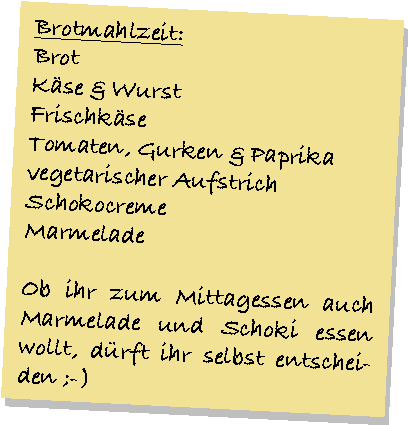
\includegraphics[center,clip=true]{note-brotmahlzeit-crop.pdf}
        
    }

    
    % \hint{%
    %     Noch Fragen? Dann lasst es Euch schmecken!
    % }
    
\end{recipe}
%!TEX root = ../Kochbuch.tex

% Complete recipe example
\begin{recipe}{Bratkartoffeln mit Sour-Cream}
    \graph{
        big=pic/kartoffeln,     % small picture
        small=pic/bratkartoffeln  % big picture
    }
    
    % \introduction{%
    %     \blindtext
    % }
    
    \ingredients{%
        \unit[2,5]{kg} & Kartoffeln \emph{(festkochend)}\\
        \unit[1,25]{kg} & Saure Sahne\\
        0,5 Knollen & Knoblauch\\
        1 Bund & Petersilie\\
        1 Bund & Schnittlauch\\
        1/4 Tube & Senf\\
        \unit[250]{g} & Zwiebeln
    }
    
    \preparation{%
        \step Die Kartoffeln sauber bürsten \emph{oder} schälen, in Scheiben oder Würfel schneiden (die ganz Verrückten können auch beides machen!) und 5 Minuten in kaltes Wasser einlegen. 
        \step Kartoffeln herausnehmen und beginnen, sie bei kleiner Stufe in Öl anzubraten. Einen Deckel aufzulegen ist sinnvoll, das spart Gas oder Holz. Achtet aber darauf, dass das ganze nicht zu feucht wird, sonst braten die Kartoffeln nicht richtig. Währenddessen können Zwiebeln und Knoblauch zerkleinert werden.
        \step Nach 5 Minuten können die Kartoffeln das erste Mal gewendet werden, Ihr müsst die Kartoffeln regelmäßig kontrollieren, damit sie nicht anbrennen. 
        \step Wenn die Kartoffeln anfangen, eine schön goldbraune Farbe zu bekommen, gebt je die Hälfte von Knoblauch und Zwiebeln hinzu und salzt sie ein wenig. 
        \step Wer zwischendurch Zeit hat und nur in der Küche rumsteht, kann sich die frischen Kräuter schnappen und sie fein hacken und dann gemeinsam mit der anderen Hälfte des Knoblauch-Zwiebel-Gemischs in die Sour Creme einrühren. Eine Idee Senf gibt der Sour Creme den letzten Schliff. 
Danach nur noch salzen und pfeffern und sie ist fertig.
        \step Unter regelmäßigem Wenden solltet Ihr sie so lange braten lassen, bis die Kartoffeln den gewünschten Grad an Knusprigkeit erlangt haben und die Zwiebeln glasig geworden sind. Auch hier noch je eine Prise Salz und Pfeffer (oder auch etwas mehr) hinzugeben, alles servieren und im Essenskreis anschreien. (ÜÜÜÜBEN!!!)
    }
    
    % \hint{%
    %     Enjoy typesetting recipes with {\textbf{\Large\LaTeX}} and {\textbf{\Large xcookybooky!}}
    % }
    
\end{recipe}
%!TEX root = ../Kochbuch.tex

% Complete recipe example
\begin{recipe}{Kartoffelgulasch}
    \graph{
        small=pic/kartoffelgulasch,
        big=pic/gulasch
    }
    
    % \introduction{%
    % ``Das ist vergleichsweise einfach, aber man muss viel schneiden.''\flushright --- \emph{Jack the Ripper}
    % }
    
    \ingredients{%
        750 g & Rindfleisch \emph{(Gulasch)}\\
        1 kg & Zwiebeln\\
        1 kg & Kartoffeln \emph{(mehlig)}\\
        0,5 Knollen & Knoblauch\\
        3 Stück & Paprika\\
        1 Tube & Tomatenmark\\
        1,5 Liter & Gemüsebrühe
    }
    
    \preparation{%
        \step Kartoffeln (Würfel), Zwiebeln (Ringe) und Knoblauch (fein gehackt) in etwas Öl anschwitzen und nach ca. 5 Minuten mit Gemüsebrühe ablöschen. Das Ganze 15 Minuten vor sich hin köcheln. 
        
        
        \step Jetzt kann Paprika kleingeschnitten und hinzugegeben werden. Gleichzeitig könnt Ihr beginnen, die Gulasch-Stücke in einer zweiten Pfanne scharf anzubraten: 
        
        Das bedeutet, bei großer Hitze mit etwas Öl das Fleisch schnell braten, so bleibt es saftiger.
        
        
        \step Gebt das Fleisch in den großen Topf zum Rest und schmeckt alles mit Tomatenmark, Salz und Pfeffer ab. Hui, das ist ja ein leckeres Mahl! Guten Abbo.
        
    }
    
    % \hint{%
    %     Noch Fragen? Dann lasst es Euch schmecken!
    % }
    
\end{recipe}
%!TEX root = ../Kochbuch.tex

% Complete recipe example
\begin{recipe}{Spätzle mit Linsen}
    \graph{
        small=pic/spaetzle-linsen,
        big=pic/linsen
    }
    
    % \introduction{%
    % Risotto ist DAS Gericht, das das Prädikat "{}schlotzig"{} trägt. Gemeint ist die Konsistenz, die der Reis erreichen soll und die ist genauso, wie es das Wort vermuten lässt.
    % }
    
    \ingredients{%
       1,5 kg & Spätzle\\
       600 g & Linsen \emph{(trocken)}\\
       300 g & Zwiebeln\\
       300 g & Karotten\\
       3 Stange & Lauch\\
       0,5 Stück & Knollensellerie\\
       2 Liter & Gemüsebrühe
    }
    
    \preparation{%
        \step \textbf{ACHTUNG: Die Linsen sollen am besten am Abend vorher in warmes Wasser eingelegt werden, oder die Kochzeit verlängert sich um ca. 1 Stunde!}
        
        \step Die Linsen werden in einem Topf mit dem geschnittenen Lauch, Karotten und dem fein gewürfelten Sellerie in Gemüsebrühe gekocht. Gebt in den Topf auch geviertelte Zwiebeln hinzu, das gibt mehr Geschmäckle. 
        
        Und natürlich gilt: Deckel zu, das spart Energie!
        
        \step Parallel dazu können die Spätzle nach Anleitung zubereitet werden: Wasser zum Kochen bringen, Salz rein und die Spätzle hinterher. Ab und zu umrühren, und nach etwa 8 Minuten sollten sie fertig sein.
        
        \step Wenn beides fertig ist, nehmt die Zwiebeln aus der Linsenmasse heraus. Im Essenskreis wird beides gemeinsam auf die Teller geschmissen und alle können selbst mit Salz, Pfeffer und Weißweinessig nachwürzen. 
        
        Hmmm, good old Süddeutschland.
    }

    
    \setHeadlines{hinthead = Spätzle aus'm Ländle}
    \hint{%
        Zuhause kann man Spätzle ganz leicht selbst machen: Der Teig besteht aus Eiern, Mehl, Salz und Milch. Nur für die klassische Form braucht man eine Spätzlepresse oder ein Brett zum schaben. 
    }
    
\end{recipe}
%!TEX root = ../Kochbuch.tex

% Complete recipe example
\begin{recipe}{Krautnudeln}
    \graph{
        big=pic/krautnudeln,
        small=pic/krautkopf
    }
    
    % \introduction{%
    % ``Das ist vergleichsweise einfach, aber man muss viel schneiden.''\flushright --- \emph{Jack the Ripper}
    % }
    
    \ingredients{%
        1,5 kg & Nudeln\\
        1 Kopf & Kohl\\
        500 g & Zwiebeln\\
        0,5 Knollen & Knoblauch
    }
    
    \preparation{%
        \step Als erstes werden die Zwiebeln klein geschnitten, gesalzen und in etwas Öl angeschwitzt.
        
        \step Während sie auf kleiner Stufe köcheln behandelt Ihr den Kohlkopf wie folgt:
Die Blätter, die außen liegen, werden abgemacht, der restliche Kopf wird geviertelt. Dann wird er mit einem scharfen Messer in feine Streifen geschnitten, so dass so genannte Juliennes \emph{(frz. für feine Streifen)} entstehen. Waschmaschine!
        
        Der Kohl wird, gemeinsam mit fein gehacktem Knoblauch, in den Topf mit den Zwiebeln getan. Deckel drauf, kleinste Stufe. Warten. 
        
        \step Währenddessen könnt Ihr die Nudeln kochen: Wasser zum kochen bringen, ein paar Löffel Salz rein und die Nudeln dazu.
        \step Die gekochten Nudeln zum Kraut geben, alles ordentlich durchmischen. Fertig!
        
        \step Im Essenskreis passt dazu Pfeffer und, auch wenn es komisch klingt, Zucker. Zum Portionieren des Zuckers empfiehlt sich ein kleiner Löffel. Denn ganz ehrlich, wir kennen doch unsere Kinders!?
        
    }
    
    % \hint{%
    %     Energiespartipp: Legt beim Kochen der Kartoffeln den Deckel auf den Topf und füllt diesen nur zu einem Drittel mit Wasser.
    % }
    
\end{recipe}
%!TEX root = ../Kochbuch.tex

% Complete recipe example
\begin{recipe}{Gemüseeintopf}
    \graph{
        small=pic/gemueseeintopf,
        big=pic/gemueseeintopf2,
    }
    
    % \introduction{%
    %     Sauce? Sose? Sauce? Oder Sauße? Aber Eier!
    % }
    
    \ingredients{%
        0,25 Stück & Knollensellerie\\
        3 Stück & Paprika\\
        2 Stange & Lauch\\
        500 g & Karotten\\
        500 g & Zucchini\\
        400 g & Kartoffeln (mehlig)\\
        200 g & Zwiebeln\\
        1 Tube & Tomatenmark\\
        2 Liter & Gemüsebrühe\\
        1 Laib 1kg & Schwarzbrot
    }
    
    \preparation{%
        \step Den Lauch in Ringe schneiden, Zwiebeln fein und Sellerie grob würfeln. Alles salzen und in einem Topf mit etwas Öl anbraten. 

        \step Die Kartoffeln können geschält, gewürfelt und als nächstes dazugegeben werden. 
Als nächstes sind die Karotten dran und danach kommen Paprika und Zucchini rein. 
        
        \step Wenn alles Gemüse im Topf ist, kann er mit Gemüsebrühe (Pulver und Wasser) aufgefüllt werden. Der Eintopf lässt sich gut mit Tomatenmark verfeinern. Ein guter Kanten Schwarzbrot erlaubt uns, bald satt zu sein. Mjam!

    }
    
    % \hint{%
    %     Wenn Ihr einen Deckel für das Kartoffel-Kochgefäß habt, dann habt Ihr die Möglichkeit, Energie zu sparen: Füllt den Topf nur etwa 1/3 so hoch mit leicht gesalzenem Wasser, wie Kartoffeln drin sind. Tut dann den Deckel drauf, die Kartoffeln werden schneller gar und Ihr spart Gas bzw. Holz! Wer wissen will, wie das funktioniert, fragt Kilian oder Kielius. Die können das erklären!
    % }
    
\end{recipe}
%!TEX root = ../Kochbuch.tex

% Complete recipe example
\begin{recipe}{Türkische Linsensuppe}
    \graph{
        small=pic/rote-linsen,
        big=pic/tuerkische-linsensuppe
    }
    
    \introduction{%
    ``...des mag isch ganz besonners gern...''\flushright --- \emph{Joel "{}böll"{} Fourier}, Friedberg
    }
    
    \ingredients{%
        1 kg & Linsen (rote)\\
        500 g & Zwiebeln\\
        0,5 Knollen & Knoblauch\\
        500 g & Tomaten\\
        100 g & Butter\\
        5 Liter & Gemüsebrühe\\
        1 Laib 1kg & Schwarzbrot\\
        500 g & Sahne\\
        0,5 Bund & Minze\\
        1 Stück & Zitrone\\
        0,5 Stück & Chilischote
    }
    
    \preparation{%
        \step Zunächst machen wir eine Pfefferminzbutter. Dazu wird Butter geschmolzen und die Minze darin ca. fünf Minuten geschwenkt. Oder geschwunken? Nehmt die Pfefferminzbutter aus dem Topf und gießt sie in einen kleinen Behälter.
        
        \step Jetzt könnt Ihr in Öl die klein geschnittenen Zwiebeln und den Knoblauch anschwitzen. Salzen nicht vergessen. 
        
        \step Als nächstes werft Ihr voll der Achtung für die uns hingegebenen Linsen genau diese in den Topf und füllt ihn mit der Gemüsebrühe auf. 
        
        \step Jetzt köchelt das Gericht vor sich hin, so lange, bis keine Linsen mehr zu erkennen sind. Gebt nun den Saft der Zitronen und etwas kleingehackte Schale der Bio-Zitrone hinzu und lasst es köcheln. 
        
        \step Die Tomaten und die fein gehackte Chili komplettieren das Mahl. Unter Dreingabe der Minzbutter kann die Suppe serviert werden; Dazu passt ein gutes Stück Schwarzbrot!
        
    }

    % \hint{%
    %     Manche Stimmen bezeichnen dieses Gericht als das beste Abendessen, das es heute gibt.
    % }
    
\end{recipe}
%!TEX root = ../Kochbuch.tex

% Complete recipe example
\begin{recipe}{Spinat-Sahne-Sauce mit Nudeln}
    \graph{
        small=pic/spinat-sahne-sauce,
        big=pic/spinat
    }
    
    % \introduction{%
    % Risotto ist DAS Gericht, das das Prädikat "{}schlotzig"{} trägt. Gemeint ist die Konsistenz, die der Reis erreichen soll und die ist genauso, wie es das Wort vermuten lässt.
    % }
    
    \ingredients{%
       1,3 kg & Nudeln \emph{(Vollkorn)}\\
       1,2 kg & Spinat\\
       500 g & Sahne\\
       500 g & Zwiebeln\\
       1 Knollen & Knoblauch
    }
    
    \preparation{%
        \step Zunächst werden die Nüdelchen aufgesetzt und nach Anleitung gekocht... Ihr kennt das ja - Wasser kochen, Salz dazu und dann die Nudeln dazu - ab und zu umrühren. 
        
        \step Den frischen Spinat müsst ihr vor dem Essen Waschen und dann blanchieren (sprich: blongschieren). Das bedeutet, Ihr bringt leicht gesalzenes Wasser zum Kochen und legt die Spinatblätter, die Ihr schon klein geschnitten habt, in das kochende Wasser. 
        
        \step Nach einer halben Minute fischt Ihr die Blätter wieder heraus und steckt sie zum Abkühlen in einen anderen Topf mit kaltem Wasser. Der Spinat wird sehr viel Volumen einbüßen, also habt Ihr am Ende viel weniger Kram, der in die Sauce kommt.
        
        \step Währenddessen könnt Ihr schon Zwiebeln und Knoblauch klein schneiden, salzen und in Öl anschwitzen. 
        
        \step Wenn die Zwiebeln schön glasig sind, kann der Spinat Einzug in den Kochtopf erhalten. Lasst das Ganze ca. 5 Minuten köcheln und gebt dann Sahne und Gemüsebrühe dazu. 
        
        \step Das ganze kann jetzt mit Salz, Pfeffer und Muskat abgeschmeckt werden. 
        
    }
    
    \setHeadlines{hinthead = Echt wahr!}
    \hint{%
        Manche Stimmen bezeichnen dieses Gericht als das beste Abendessen, das es heute gibt.
    }
    
\end{recipe}
%!TEX root = ../Kochbuch.tex

% Complete recipe example
\begin{recipe}{Schinken-Sahne-Sauce mit Nudeln}
    \graph{
        small=pic/schinken-sahne-sauce,
        big=pic/nudeln
    }
    
    % \introduction{%
    % Risotto ist DAS Gericht, das das Prädikat "{}schlotzig"{} trägt. Gemeint ist die Konsistenz, die der Reis erreichen soll und die ist genauso, wie es das Wort vermuten lässt.
    % }
    
    \ingredients{%
       1,3 kg & Nudeln (Vollkorn)\\
       500 g & Schinken\\
       500 g & Zwiebeln\\
       1 Knollen & Knoblauch\\
       700 g & Sahne\\
       400 g & Crème fraîche\\
       1 Bund & Petersilie\\
       2 Bund & Schnittlauch
    }
    
    \preparation{%
        \step Als erstes könnt Ihr die Nudeln nach Anleitung al dente kochen. Wir haben keine Ahnung, was das bedeutet, es klingt aber wahnsinnig gut. Schaut mal nach links, da ist es auch nochmal genau erklärt...
        
        \step Die Zwiebeln und der Knoblauch werden gewürfelt bzw. fein gehackt, gesalzen und in etwas Öl angeschwitzt. 
        
        \step Wenn sie schön glasig sind, dann wird der Schinken, den Ihr vorher in feine Streiflein geschnitten habt, zugegeben. 
        
        \step Danach kann Sahne und Crème Fraîche der Mixtur hinzugefügt werden. Würzt das Ganze mit Salz, Pfeffer und Muskatnuss. 
        
        \step Zum Schluss werden die Petersilie und der (oder das?) Schnittlauch zugeführt. Mit den frisch gekochten Nudeln ergibt sich ein leckeres Hauptgericht. 
        
    }
    %
    % \hint{%
    %     In einigen Stämmen werden ähnliche Gerichte - gegebenenfalls auch ungekocht - unter dem Namen "{}Ingelschleim"{} angepriesen. Aus Gründen der Diskretion gehen wir hier aber nicht näher auf die betroffenen Gruppen ein.
    % }
    
\end{recipe}
%!TEX root = ../Kochbuch.tex

% Complete recipe example
\begin{recipe}{Eier in Senfsauce}
    \graph{
        small=pic/eier-in-senfsosse,
        big=pic/eier
    }
    
    \introduction{%
        Sauce? Sose? Soße? Oder Sauße? Aber Eier!
    }
    
    \ingredients{%
        20 & Eier\\
        2,5 kg & Kartoffeln\\
        50 g & Butter\\
        100 g & Mehl\\
        200 g & Sahne\\
        0,5 Liter & Milch\\
        2 Glas & Senf \emph{(á 200g)}\\
    }
    
    \preparation{%
        \step Stellt als erstes die geschälten (oder für die fauleren Stämme: gewaschenen) Kartoffeln aufs Feuer. 

        \step Danach könnt Ihr die Eier aufstellen. Wer keinen Anpiekser dabei hat: Gar nicht schlimm. Anstatt irgendwie mit einem Hering ein Loch reinzupulen, lasst sie lieber ganz. Das gefällt den Eiern besser. Etwa 7 Minuten nachdem das Wasser kocht, könnt Ihr die Eier herausnehmen und dann warten sie bestimmt gern auf die anderen Komponenten des Essens.
        
        \step Die [s'oußä] wird folgendermaßen hergerichtet: Erhitzt die Butter in einem Topf und schwitzt darin die klein geschnittenen Zwiebeln an. Wenn die schön glasig sind, fügt langsam und unter stetigem Rühren das Mehl hinzu. Es entsteht eine Mehlschwitze, jetzt schnell (!) Milch und Sahne hinzu und, je nach Geschmack, ein bisschen Gemüsebrühe-Pulver. Wichtig: immer weiter rühren!
        
        \step Die Sauce wird schön dick und kann jetzt mit Senf, Muskatnuss (bitte gerieben) und Salz und Pfeffer abgeschmeckt werden. 
        
        \step Sind die Kartoffeln auch schon fertig? Dann legt das Kochbuch beiseite und nehmt im Essenskreis Platz, bevor es kalt wird. Und Eier nicht vergessen!
    }
    
    
    \setHeadlines{hinthead = Kilian's Trick}
    \hint{%
        Wenn Ihr einen Deckel für das Kartoffel-Kochgefäß habt, dann habt Ihr die Möglichkeit, Energie zu sparen: Füllt den Topf nur etwa 1/3 so hoch mit leicht gesalzenem Wasser, wie Kartoffeln drin sind. Tut dann den Deckel drauf, die Kartoffeln werden schneller gar und Ihr spart Gas bzw. Holz! Wer wissen will, wie das funktioniert, fragt Kilian oder Kielius. Die können das erklären!
    }
    
\end{recipe}
%!TEX root = ../Kochbuch.tex

% Complete recipe example
\begin{recipe}{Grüne Sauce mit Kartoffeln}
    \graph{
        small=pic/gruene-sauce,
        big=pic/gruene-kaeuter
    }
    
    \introduction{%
    ``Das ist vergleichsweise einfach, aber man muss viel schneiden.''\flushright --- \emph{Jack the Ripper}
    }
    
    \ingredients{%
        1 Bund & Petersilie\\
        1 Bund & Schnittlauch\\
        0,5 Bund & Pimpinelle\\
        0,5 Bund & Sauerampfer\\
        0,5 Bund & Kerbel\\
        0,5 Bund & Borretsch\\
        1 Pack & Kressesamen\\
        2,5 kg & Kartoffeln\\
        1 kg & Saure Sahne\\
        15 & Eier\\
    }
    
    \preparation{%
        \step Die Kartoffeln können, wie immer, geschält oder nur gewaschen werden. In einem Topf könnt Ihr sie kochen; ihr verbraucht weniger Energie, wenn Ihr den Deckel auf den Topf setzt und ihn nur zu einem Drittel mit gesalzenem Wasser füllt.
        
        \step Die Kräuter, die Ihr jeweils an den Kräuterstationen in Eurer Nähe gesammelt habt, werden kleingeschnitten (sehr fein Hacken gibt der Soße am Ende eine grüne Farbe) und mit der Sauren Sahne vermischt. 
        
Die Eier werden hart gekocht, kleingeschnitten und ebenfalls unter die Soße gemengt.
    }
    
    
    \setHeadlines{hinthead = Fun Fact}
    \hint{%
        Es ist nicht sicher erwiesen, dass Johann Wolfgang von Goethe wirklich dasselbe Rezept für Frankfurter Grüne Soße als sein Leibgericht bezeichnet hat. Was für ein armer Tor.
    }
    
\end{recipe}
%!TEX root = ../Kochbuch.tex

% Complete recipe example
\begin{recipe}{Kartoffelsalat aus Lettland}
    \graph{
        big=pic/kartoffelsalat,
        small=pic/kartoffeln
    }
    
    % \introduction{%
    % ``Das ist vergleichsweise einfach, aber man muss viel schneiden.''\flushright --- \emph{Jack the Ripper}
    % }
    
    \ingredients{%
        4 kg & Kartoffeln \emph{(festkochend)}\\
        10 Stück & Eier\\
        1 kg & Saure Sahne\\
        500 g & Saure Gurken\\
        300 g & Crème fraîche\\
        2 Bund & Dill\\
        200 g & Frühlingszwiebeln\\
        etwas & Senf
    }
    
    \preparation{%
        \step Die Kartoffeln können als erstes geschält und in Würfel oder Scheiben geschnitten werden. Kocht sie ca. 15 Minuten lang in gesalzenem Wasser und gießt sie ab, wenn sie gar sind.
        
        Das solltet ihr ruhig auch schon lange vor dem Essen machen - soll ja kalt werden.
        
        \step Verfahrt ebenso mit den Eiern, aber schneidet sie erst nach dem Kochen in Würfel :-) Die Eier brauchen ca. 7 Minuten. Aber lieber etwas zu lang als zu kurz.        
        
        \step Die klein geschnittenen Gurken mit Saurer Sahne, Dill (gehackt), klein geschnittenen Frühlingszwiebeln, Eiern und Kartoffeln zusammenmischen. Gebt noch einen ordentlichen Schluck von dem Gurkenwasser dazu, das gibt dem Salat eine feinsaure Note.
        
        \step Mit Senf, Salz und Pfeffer abschmecken und Ihr habt ein köstliches Stück Baltikum zubereitet. Lasst es Euch schmecken!
        
    }
    
    \setHeadlines{hinthead = *pssst* Küchengeheimnis}
    \hint{%
        Energiespartipp: Legt beim Kochen der Kartoffeln den Deckel auf den Topf und füllt diesen nur zu einem Drittel mit Wasser.
    }
    
\end{recipe}
%!TEX root = ../Kochbuch.tex

% Complete recipe example
\begin{recipe}{Käsespätzle}
    \graph{
        big=pic/kaesespaetzle,
        small=pic/spaetzle-zutaten
    }
    
    % \introduction{%
    % ``Das ist vergleichsweise einfach, aber man muss viel schneiden.''\flushright --- \emph{Jack the Ripper}
    % }
    
    \ingredients{%
        1,5 kg & Spätzle\\
        400 g & Emmentaler \emph{(gerieben)}\\
        100 g & Gruyere\\
        600 g & Zwiebeln\\
        50 g & Butter\\
        300 g & Crème fraîche
    }
    
    \preparation{%
        \step Die Zwiebeln werden kleingeschnitten und gesalzen. Bei kleiner Flamme werden sie jetzt in Butter angeschwitzt, bis sie schön glasig sind. Wenn sie eine schön flutschige Konsistenz haben, können sie beiseite genommen werden.
        
        \step Jetzt kommen die Spätzle dran: In einem Topf mit gesalzenem Wasser werden die Spätzle nach Anleitung gekocht. Wer noch nicht weiß, wie das geht kann auf Seite 14 blättern, da ist es erklärt...      
        
        \step Wenn die Spätzle fertig sind: abschütten und danach mit dem geriebenen oder klein gehackten Käse in einem großen Topf oder Schüssel vermischt. 
        
        \step Die Zwiebeln werden auch dazugegeben und der Schmand kann entweder so reingemischt oder im Essenskreis zum Selber-Portionieren hingestellt werden.
        
        Käsespätzle vs. Risotto - schwere Wahl...
        
    }
    
    % \hint{%
    %     Energiespartipp: Legt beim Kochen der Kartoffeln den Deckel auf den Topf und füllt diesen nur zu einem Drittel mit Wasser.
    % }
    
\end{recipe}
%!TEX root = ../Kochbuch.tex

% Complete recipe example
\begin{recipe}{Risotto}
    \graph{
        small=pic/risotto,
        big=pic/risottoreis
    }
    
    \introduction{%
    Risotto ist DAS Gericht, das das Prädikat "{}schlotzig"{} trägt. Gemeint ist die Konsistenz, die der Reis erreichen soll, und die ist genau so, wie es das Wort vermuten lässt.
    }
    
    \ingredients{%
        1 kg & Risotto Reis\\
        800 g & Champignons\\
        500 g & Zwiebeln\\
        200 g & Butter\\
        2 Liter & Gemüsebrühe\\
        1 Bund & Petersilie\\
        300 g & Parmesan (gehobelt)
    }
    
    \preparation{%
        \step Als erstes müssen die Zwiebelchen klein geschnitten werden und in der Butter bei kleiner Flamme angeschwitzt werden. 
        
        \step Jetzt kommt der Coup (frz. für Kuh): Der Reis wird jetzt in den Topf gegeben und ein wenig angebraten, bis er überall schön glänzt. 
        
        \step Unter ständigem Rühren wird immer eine kleine Menge (ca 1-2 Fjellis) Gemüsebrühe dazugegeben. Wartet immer so lange, bis die Flüssigkeit ganz aufgesogen ist, bis Ihr das nächste Mal Brühe in den Topf schüttet. 
        
        \step Das Ganze wird so lange durchgeführt, bis der Reis schön schlotzig (bissfest-schleimig-cremig) ist. 
        
        \step Jetzt können die klein geschnittenen Champignons hinzugegeben werden, Paprika und Tomaten dazu, ein klein wenig weiter köcheln lassen und mit etwas Tomatenmark, Salz und Pfeffer abschmecken.
        
        \step Am Ende die Petersilie klein hacken und genau wie den Parmesan unterrühren. Fix servieren und die Stämme beneiden, die Käsespätzle essen... Zumindest Jonas und Kilian sind auf der Käseseite des Lebens, Anni würde immer Risotto wählen!
        
    }
    %
    % \hint{%
    %     In einigen Stämmen werden ähnliche Gerichte - gegebenenfalls auch ungekocht - unter dem Namen "{}Ingelschleim"{} angepriesen. Aus Gründen der Diskretion gehen wir hier aber nicht näher auf die betroffenen Gruppen ein.
    % }
    
\end{recipe}
%!TEX root = ../Kochbuch.tex

% Complete recipe example
\begin{recipe}{Milchreis}
    \graph{
        big=pic/milchreis,
        small=pic/obst
    }
    
    % \introduction{%
    % ``Das ist vergleichsweise einfach, aber man muss viel schneiden.''\flushright --- \emph{Jack the Ripper}
    % }
    
    \ingredients{%
        2,5 Liter & Milch\\
        625 g & Milchreis\\
        3 Stück & Apfel\\
        3 Stück & Bananen\\
        3 Stück & Birnen\\
        100 g & Zucker
    }
    
    \preparation{%
        \step Zuerst wird die Milch aufgekocht. Achtet hier drauf, dass Ihr viel umrührt, dass die Milch nicht anbrennen kann. 
        
        \step Wenn die Milch kocht, dann schmeißt den Zucker rein und den Reis dazu. Jetzt ist das Umrühren noch wichtiger. 
        
        \step Lasst den Deckel drauf, um schon wieder Energie zu sparen. Und wenn der Milchreis schön saftig lecker ist, dann kann er serviert werden.
        
        \step Mit etwas Zimt und dem geschnittenen Obst habt Ihr ein feini feini Fress'chen.
        
    }
    
    % \hint{%
    %     Energiespartipp: Legt beim Kochen der Kartoffeln den Deckel auf den Topf und füllt diesen nur zu einem Drittel mit Wasser.
    % }
    
\end{recipe}

\newpage
\section{Küchen-SOS - Was tun, wenn...}
\subsection*{... zu viel Salz im Essen gelandet ist?} % (fold)
\label{sub:_zu_viel_salz_im_essen_gelandet_ist}
\begin{itemize}
    \item Bei einer Suppe oder einem Eintopf könnt ihr einfach eine Kartoffel oder etwas Reis (am besten im Teebeutel) mit kochen und so das Salz wieder rausziehen. 
    \item Bei Soßen könnt ihr auch noch etwas Wasser hinzugießen und es einfach n bisschen länger einkochen lassen.
\end{itemize}
% subsection _zu_viel_salz_im_essen_gelandet_ist (end)

\subsection*{... das Essen unten anbrennt?} % (fold)
\label{sub:_das_essen_unten_anbrennt}
\begin{itemize}
    \item Einfach alles, was noch nicht verbrannt ist, in einen neuen Topf geben. Vorsichtig abheben.
\end{itemize}
% subsection _das_essen_unten_anbrennt (end)

\subsection*{... der Kräutergarten leer ist?} % (fold)
\label{sub:_der_krautergarten_leer_ist}
\begin{itemize}
    \item Das ist erstmal doof! Deswegen gilt: Nehmt bitte nur so viel, wie ihr auch braucht. Wenn ihr den kleinen Garten fleißig gießt und pflegt, sollte bald wieder etwas da sein. Bis dahin gibt es eben nur getrocknete Kräuter.
    \item Keine Panik: Die Kräuter für die Grüne Soße kriegt ihr von uns direkt.
\end{itemize}
% subsection _der_krautergarten_leer_ist (end)

\subsection*{... ihr das Gefühl habt, ihr kriegt zu wenig Fleisch zu den Hauptmahlzeiten?} % (fold)
\label{sub:_ihr_das_gefuhl_habt_ihr_kriegt_zu_wenig_fleisch_zu_den_hauptmahlzeiten}
\begin{itemize}
    \item Also erstmal: Wir haben uns ja was überlegt bei unserem Verpflegungskonzept und es ist garnicht gesund, jeden Tag Fleisch zu essen. Aber für die, die garnicht damit zurecht kommen: Man könnte ja einfach ein wenig Wurst von den Brotzeiten abzwacken und so die Hauptmahlzeiten verfeinern.
\end{itemize}
% subsection _ihr_das_gefuhl_habt_ihr_kriegt_zu_wenig_fleisch_zu_den_hauptmahlzeiten (end)

\subsection*{... wenn's brennt?} % (fold)
\label{sub:_wenn_s_brennt}
\begin{itemize}
    \item Ruhig bleiben und löschen – in heißes Fett kein Wasser kippen!!!!
\end{itemize}
% subsection _wenn_s_brennt (end)

\newpage
\section{\cancel{Un}nützliches Küchenwissen}
\begin{itemize}
    \item Unsere Sipplinge trinken keinen Tee – jaja das hört man immer wieder, aber was ist mit Eistee? Den liebt ja wohl jedes Kind.

    Einfach einen großen Topf Tee kochen, Holundersirup, Zitronensaft und Minze einrühren und abkühlen lassen. Kalt ein Gedicht, wenn dann noch was da ist – warm ist es nämlich auch klasse.
    Achtung: Holundersirup und Zitronensaft gibt’s nicht von uns, aber beim Sondereinkauf oder einfach von zu Hause.
    
    \item Wenn man das Spülwasser auf kleiner Flamme bereits dann aufsetzt, wenn man zum Essen geht, kann man direkt im Anschluss spülen. Natürlich den Deckel nicht vergessen.
 
    \item Oft essen Vegetarier, Veganer und Omnivoren ja fast dasselbe – bis auf die kleinen, feinen, fleischigen Details. Oft kann man die aber einfach später in den Topf werfen, so dass ihr erstmal für alle das Gleiche kocht, dann aufteilt und perfektioniert. Viel weniger Arbeit.

    \item „Ihhhh Gurken“ hört man es aus dem Nachbarstamm schreien und wünscht sich eben diese, weil im eigenen Essenskreis keine mehr da ist. \emph{Let's swap}, sag ich da nur. Bringt Lebensmittel, die bei euch im Stamm keiner mag zum Tausch/Swap-Regal bei der Verpflegung und nehmt euch mit, was anderen nicht schmeckt. 
Aber Leute: Bitte nur Sachen, die noch im Rohzustand sind, nix gekochtes – damit läuft man über den Platz und bietet es hungrigen Stämmen an.

    \item Tauschen solltet ihr auch unbedingt bei Marmeladen. Von uns bekommt ihr keine, aber Marmelade gibt’s für alle – von euch daheim in Liebe gekocht und mit aufs Lager gebracht. Übrigens auch 'n super Tip, um endlich den Schwarm aus dem Nachbarstamm kennenzulernen: frag ihn doch einfach, ob sie oder er deine Marmelade probieren möchte.
 
    \item Für die richtigen Klugscheißer unter uns – wusstet ihr eigentlich, dass ...
    \begin{itemize}
        \item ...Brot länger frisch bleibt, wenn es am Stück ist?
        \item ...Salat und Dressing am besten getrennt serviert werden sollten, damit man beides noch aufheben kann?
        \item ...Wasser schneller kocht, wenn der Deckel drauf ist?
        \item ...man mit Reis und einem Topf zaubern kann (der Trick ist im Heft versteckt)?
        \item ...man sich eigene Kühlschränke bauen kann?
        \item ...man Wasser besser erst salzen sollte, wenn es kocht?
        \item ...Rollgerste 1000[..]00 mal besser ist als Reis (nähere Infos bei Jo aus Grävenwiesbach)?
        \item ...Kinder alles essen, wenn man ihm coole Namen gibt? \emph{„Das sind keine Krautnudeln – das sind Kraftspätzle mit magischem Kraut“}
        \item ...es gaaaaanz, gaaaanz viele Tschairezepte gibt und alle das anders machen?
        \item ...
    \end{itemize}
\end{itemize}
%!TEX root = ./Kochbuch.tex

% \section{Zeitliche Übersicht}
\definecolor{mygray}{gray}{0.70}

% Use pseudo-section to save space
\refstepcounter{section}
\addcontentsline{toc}{section}{\protect\numberline{\thesection}Zeitliche Übersicht}
\sectionmark{Zeitliche Übersicht}
% \rowcolor{mygray}

\begin{sidewaystable}
\def\arraystretch{1.3}
\begin{tabular}{ll|l|l|l|l|}
\multicolumn{1}{l|}{}            & Mi, 20. Juni       & Do, 21. Juni                                                              & Fr, 22. Juni                                                                  & Sa, 23. Juni                                                                             & So, 24. Juni                                                             \\ \hline
\rowcolor{mygray}\multicolumn{1}{l|}{Frühstück}   & -                  & Brötchenfrühstück                                                             & \begin{tabular}[c]{@{}l@{}}Brot\\ Porridge\end{tabular}                   & \begin{tabular}[c]{@{}l@{}}Brotfrühstück\\ Müsli\end{tabular}                            & Brötchenfrühstück                                                        \\ \hline
\multicolumn{1}{l|}{Mittagessen} & -                  & Griechischer Salat                                                              & Gemischter Salat mit Brot                                                   & Gemischter Salat mit Brot                                                                     & \begin{tabular}[c]{@{}l@{}}Spätzle mit Linsen\\ Krautnudeln\end{tabular} \\ \hline
\rowcolor{mygray}\multicolumn{1}{l|}{Abendessen}  & Würstchen mit Brot & \begin{tabular}[c]{@{}l@{}}Nudeln in Schinken- \\ oder Spinat-Sahne-Soße\end{tabular} & \begin{tabular}[c]{@{}l@{}}vegetarisches Curry\\ Chili sin Carne\end{tabular} & \begin{tabular}[c]{@{}l@{}}\begin{tabular}[c]{@{}l@{}}Röstkartoffeln\\ ~~~mit Sour Cream\end{tabular}\\ Kartoffelgulasch\end{tabular} & Hajkverpflegung                                                          \\ \hline
\\
\\
\\
\\
\multicolumn{1}{l|}{}             & Mo, 25. Juni                                                                  & Di, 26. Juni                                                                          & Mi, 27. Juni                                                            & Do, 28. Juni                                                             & Fr, 29. Juni \\ \hline
\rowcolor{mygray}\multicolumn{1}{l|}{Frühstück}   & Müsli                                                                         & Brötchenfrühstück                                                                     & \begin{tabular}[c]{@{}l@{}}Brotfrühstück\\ Müsli\end{tabular}           & \begin{tabular}[c]{@{}l@{}}Brotfrühstück\\ Porridge\end{tabular}         & Brunch   \\ \hline
\multicolumn{1}{l|}{Mittagessen} & Gurkensalat                                                         & (Lunchpaket)                                                                          & (Lunchpaket)                                                            & Kartoffelsalat                                                           & Milchreis   \\ \hline
\rowcolor{mygray}\multicolumn{1}{l|}{Abendessen}  & \begin{tabular}[c]{@{}l@{}}Gemüseeintopf\\ Türkische Linsensuppe\end{tabular} & \begin{tabular}[c]{@{}l@{}}Bolognese\\ vegetarisch Bolognese\end{tabular} & \begin{tabular}[c]{@{}l@{}}Grüne Sauce\\ Eier in Senfsauce\end{tabular} & \begin{tabular}[c]{@{}l@{}}Käsespätzle\\ Risotto mit Pilzen\end{tabular} & Gemeinsames Festmahl             \\ \hline
\end{tabular}
\end{sidewaystable}

\end{document}